\graphicspath{{figures/results/}}
\chapter{Results}
%The results presented are made by labelling all occlusions happening in the data. This covers the two videos provided by Loligo Systems which include three and five fish, each just about one minute long. The labelling is done by marking the point in which an occlusion is spotted, with skeletons drawn on each image. The frames of the video in which no occlusions occur does not have any labelling.
%
\section{Training}

\begin{figure}[H]
	\centering
	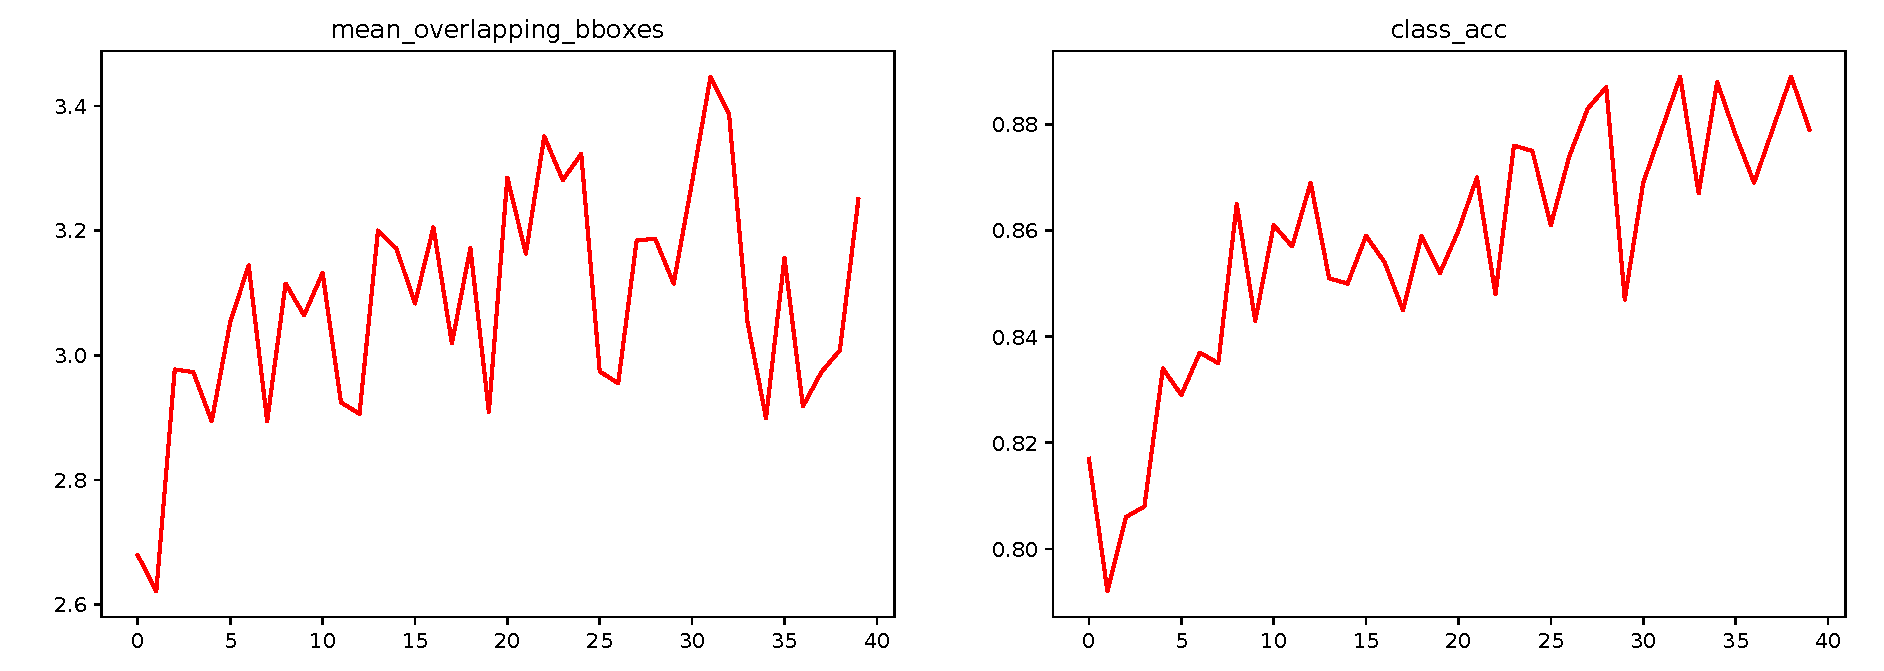
\includegraphics[width=\textwidth]{acc}
	\caption{Accuracy}
	\label{fig:}
\end{figure}
\begin{figure}[H]
	\centering
	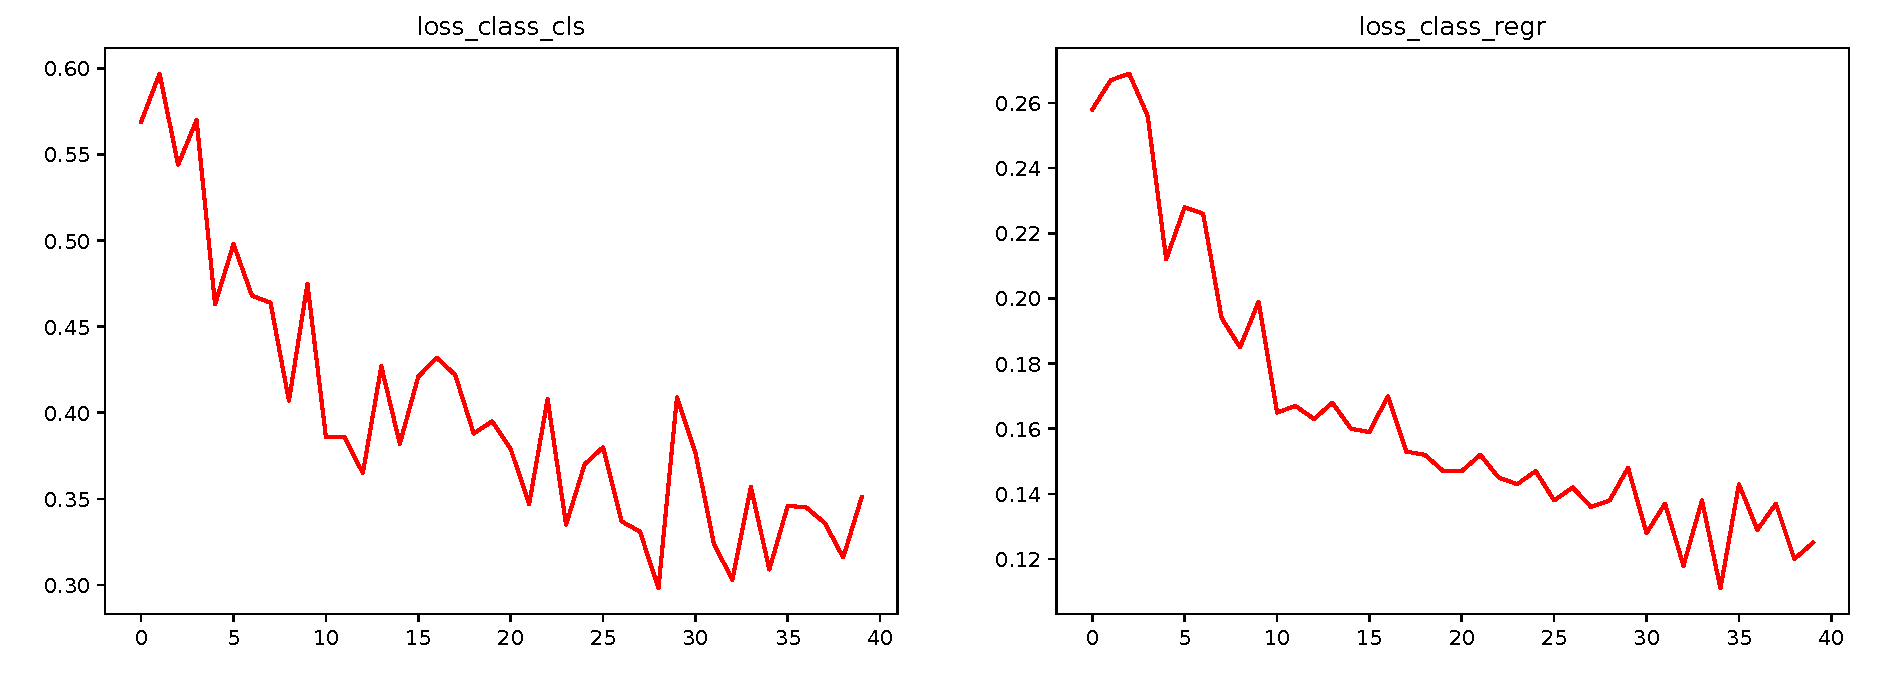
\includegraphics[width=\textwidth]{loss_class}
	\caption{Loss Class - classification and bbox regression}
	\label{fig:}
\end{figure}
\begin{figure}[H]
	\centering
	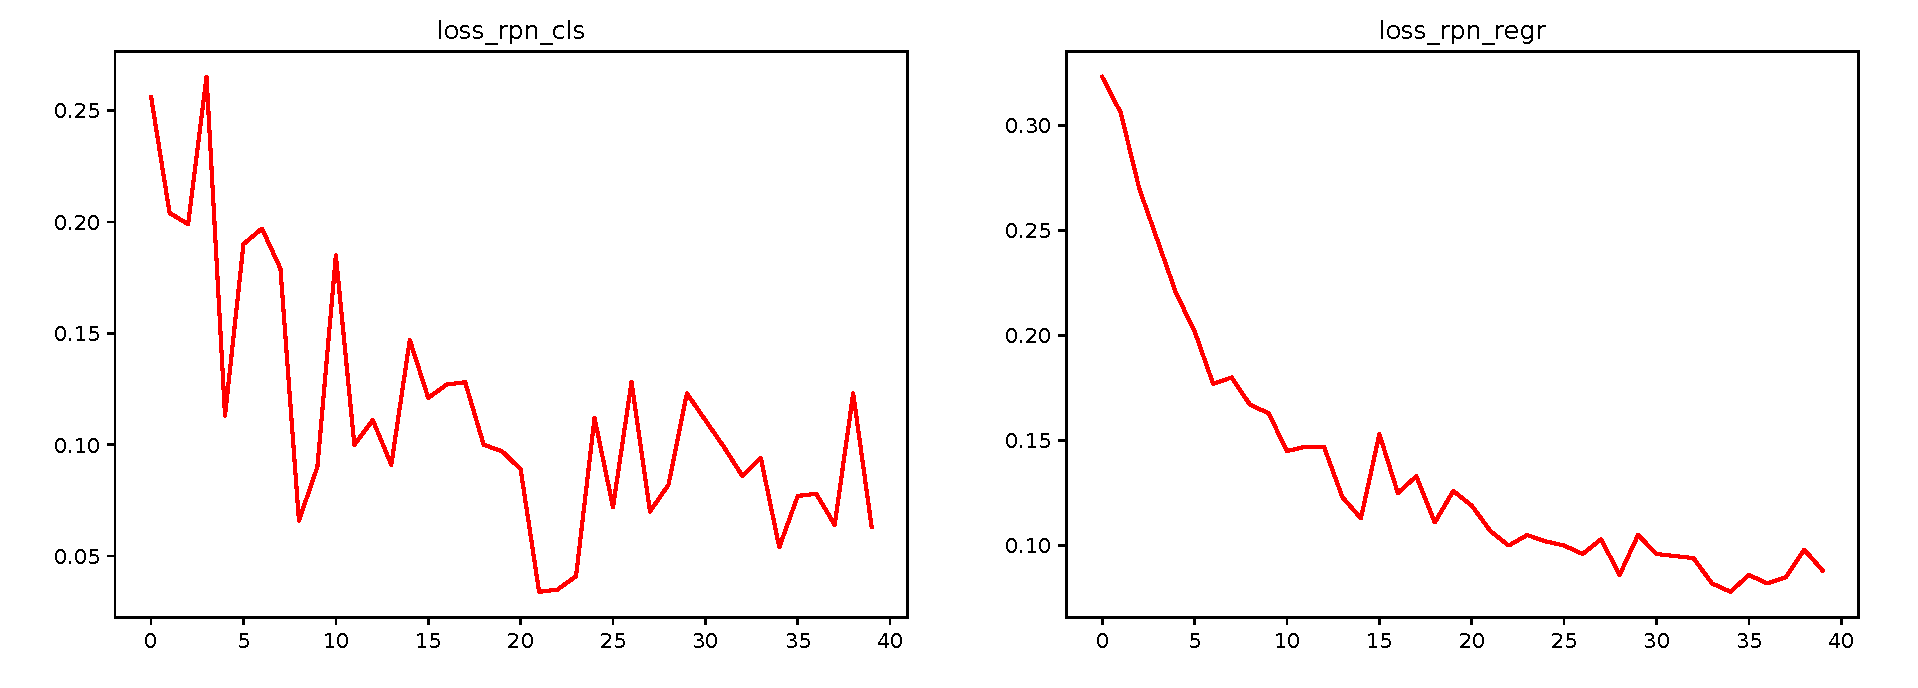
\includegraphics[width=\textwidth]{loss_rpn}
	\caption{Loss Region Proposal Network - classification and bbox regression}
	\label{fig:}
\end{figure}
\begin{figure}[H]
	\centering
	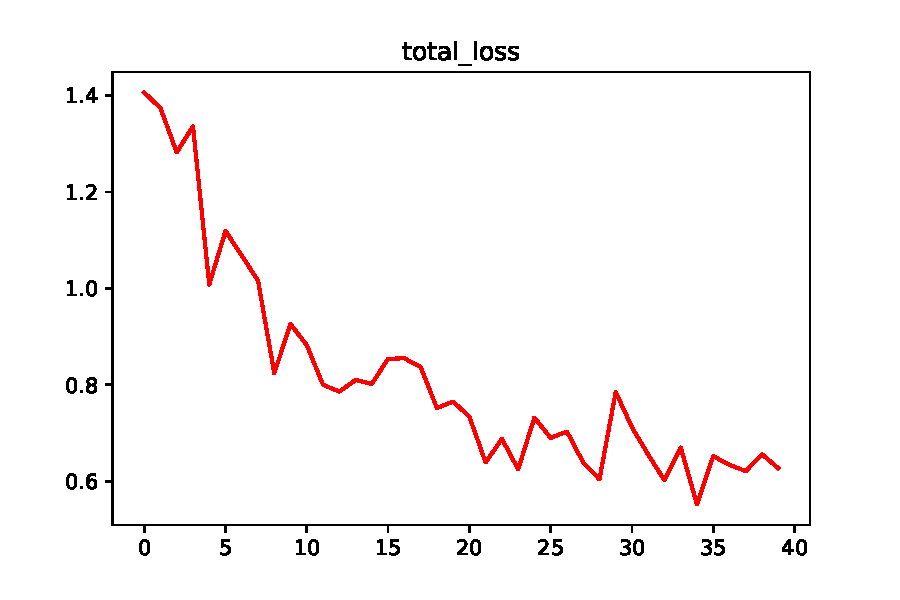
\includegraphics[width=0.85\textwidth]{total_loss}
	\caption{Total loss}
	\label{fig:}
\end{figure}

\section{Testing}
\gls{map} at $81.7\%$. \todo{Make figures showing detections}

%
%\section{Five Fish}